\documentclass[11pt, a4paper]{article}

\usepackage{amsmath}
\usepackage{amsfonts} %Matheschriften
\usepackage{amssymb} %Mathesymbole
%\usepackage{mathptmx} % Einstellung für Schriften und Sonderzeichen in mathematischen Umgebungen
                        % ändert SChriftfont
\usepackage{wasysym} % Stellt diverse Sonderzeichen bereit
\usepackage{siunitx}
\usepackage{float}
\usepackage{microtype}
\usepackage{graphicx}
\usepackage{hyperref}
\usepackage{xcolor}
\usepackage[section]{placeins}
% allows for temporary adjustment of side margins
\usepackage{changepage}
\usepackage{rotating}


\usepackage[ngerman]{babel}
\addto\captionsngerman{%
 \renewcommand{\abstractname}{Einleitung}}

\title{Versuch 4: Magnetismus}
\author{Team 2-13: Jascha Fricker, Benedict Brouwer}

\begin{document}
    \maketitle

    \tableofcontents

    \newpage

    \section{Einleitung}

    In diesem Versuch werden die Eigenschaften des Magnetfelds einer Spule mittels einer Hall-Sonde untersucht. Dabei wird der Einfluss verschiedener Ströme und eines Metallkerns gemessen.

    \section{Theorie}

    Nach dem Biot-Savart-Gesetz kann das Magnetfeld $(x)$ auf der Symmetrieachse einer dünnen Ringspule mit Radius $R$ durch die Formel
    \begin{align}
        B(x) = \frac{\mu_0 \mu_r N}{2} \cdot \frac{R^2 I}{\left(x^2 + R^2\right)^{\frac{3}{2}}} \label{eq:BiotSavart}
    \end{align}
    beschreiben werden. Dabei durchfließt die Spule eine Stromstärke $I$ mit einer Windungszahl $N$. Das Material in der Spule hat eine Permeabilität $\mu_r$ (bei Luft $\mu_r = 1$).
    
    Durch Umstellung der Gleichung nach $x$ können bei gegebenem $B_{max}$ die Spulenränder
    \begin{align}
        x_{min, \ max} = \pm \sqrt{\left(\frac{\mu_0 \mu_r N}{2} \cdot \frac{R^2 I}{B_{max}}\right)^\frac{2}{3} - R^2} \label{eq:bmax}
    \end{align}
    bestimmt werden. 

    \section{Ergebnisse und Diskussion}
    \subsection{longitudinale Konfiguration}
    Die rohen Messwerte der 4x3 verschiedenen Messreihen der longitudinalen Konfiguration wurden im Graph \ref{fig:longmess} geplottet.
    \begin{figure}[h]
        \centering
        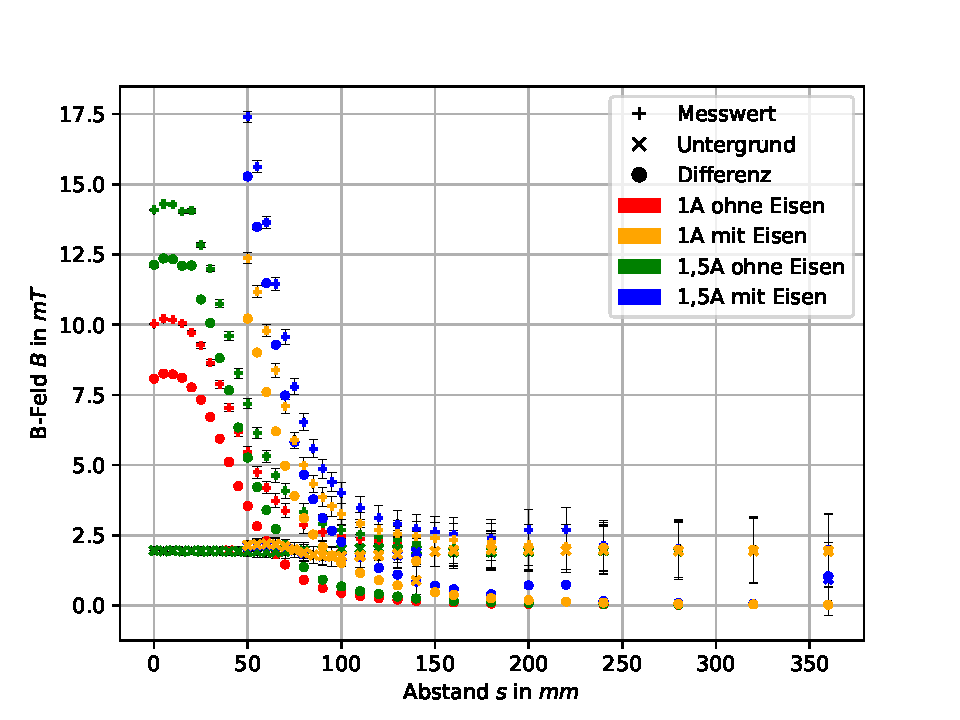
\includegraphics[width=0.9\textwidth]{raw1.pdf}
        \caption{Messwerte der longitudinalen Konfiguration}
        \label{fig:longmess}
    \end{figure}

    Im Plot \ref{fig:longfit1a} wurde die Magnetfeldstärke abzüglich der Hintergrundmagnetisierung aufgetragen und gespiegelt. Anschließend wurde die Funktion \ref{eq:BiotSavart} auf die Messwerte außerhalb der Spule gefittet und auch aufgetragen. Mit einem abgelesenen $B_{max}$ und den gefitteten parametern wurden die Spulenränder berechnet. Diese werden als vertikale Balken in dem Graphen dargestellt. Die Ergebnisse des Fits und die errechneten Werte sind in Tabelle \ref{tab:fit} aufgelistet. Die gleiche Auswertung der Messreihe mit 1,5A Stromstärke ist im Graph \ref{fig:longfit15a} dargestellt.
    
    Bei beiden Messreihen ist es erstaunlich, wie stark $I_{eff}$ von der eingestellten Stromstärke abweicht. Die Abweichung ist aber bei beiden Messreihen in sich konsistent. Auch der gefittete Radius $R_eff$ ist bei beiden Messreihen konsistent. Nur die Länge der Spule ist bei unterschiedlich. Dies kann aber auch daran liegen, dass die Abweichungen vom Biot-Savart-Gesetz mit der Stromstärke skalieren, und so der homogene Bereich des Magnetfeldes größer wird.
    \begin{table}[h]
        \centering
        \begin{tabular}{c | c | c}
            \textbf{Parameter} & \textbf{Wert mit 1A} & \textbf{Wert mit 1,5A} \\
            \hline
            $B_{max}$ & $8,26 \si{\milli\tesla}$ & $12,3 \si{\milli\tesla}$ \\
            $R_{eff}$ & $35,6 \si{\milli\metre}$ & $35,8 \si{\milli\metre}$ \\
            $I_{eff}$ & $0,74 \si{\ampere}$ & $1,10 \si{\ampere}$ \\
            $x_{min}$ & $25,9 \si{\milli\meter}$ & $35,8 \si{\milli\meter}$ \\
            $x_{max}$ & $-25,9 \si{\milli\meter}$ & $-35,8 \si{\milli\meter}$ \\
        \end{tabular}
        \caption{Ergebnisse Aufgabe 5.2.2}
        \label{tab:fit}
    \end{table}

    \begin{figure}
        \centering
        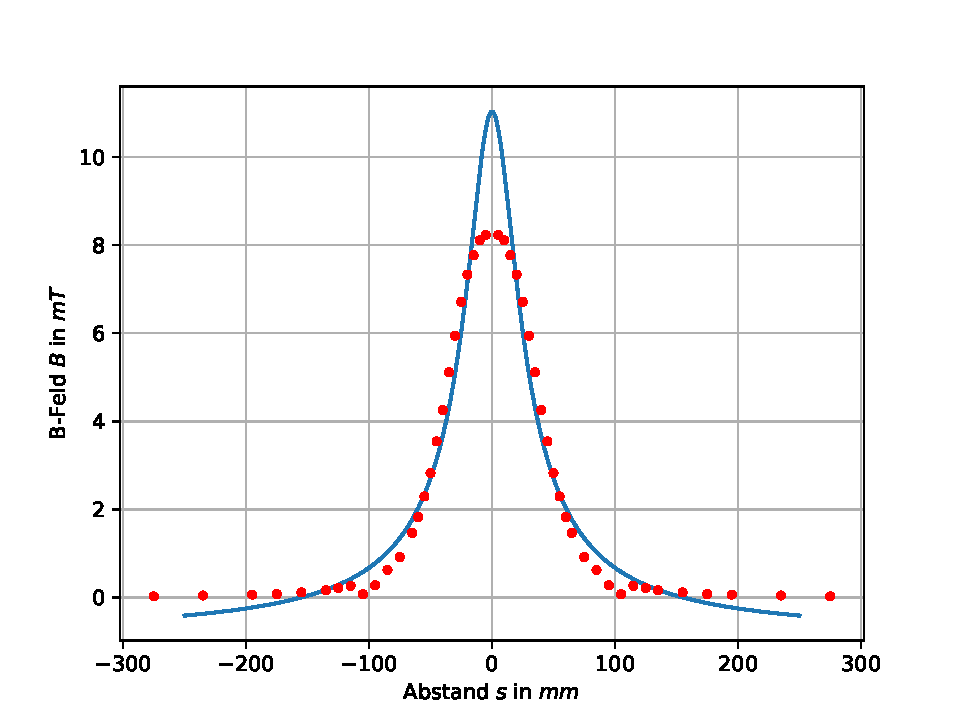
\includegraphics[width=0.8\textwidth]{fit1.pdf}
        \caption{Fit der longitudinalen Konfiguration 1 Ampere}
        \label{fig:longfit1a}
    \end{figure}

    \begin{figure}
        \centering
        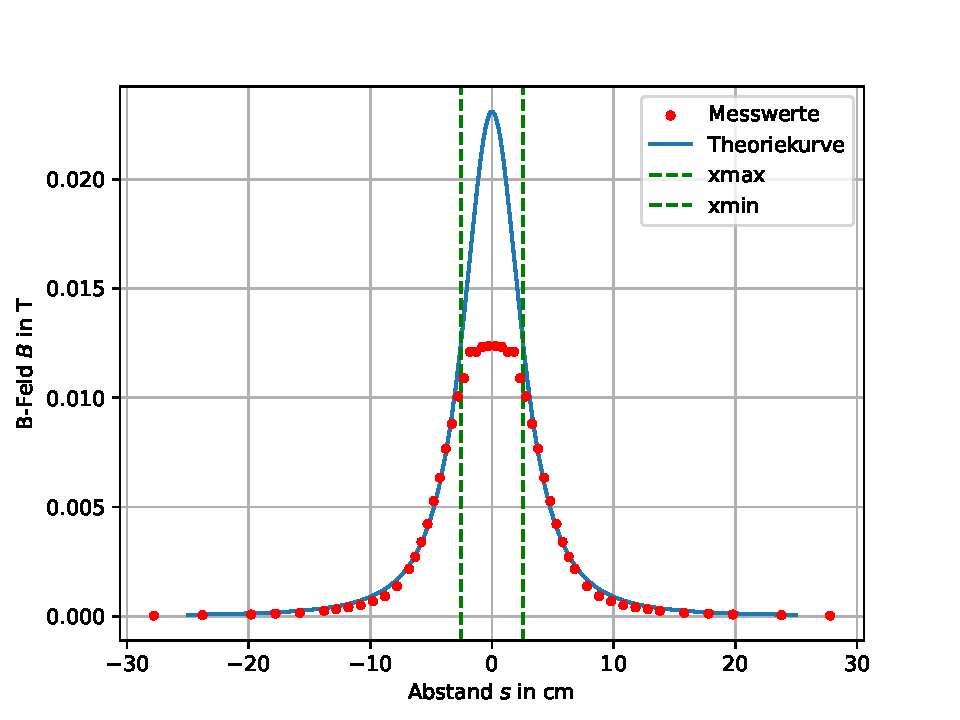
\includegraphics[width=0.8\textwidth]{fit15a.pdf}
        \caption{Fit der longitudinalen Konfiguration 1,5 Ampere}
        \label{fig:longfit15a}
    \end{figure}

    \subsection{Bestimmung von $\mu_r$}
    Mit den in \ref{tab:fit} aufgelisteten Ergebnissen, kann die Funktion \ref{eq:BiotSavart} mit einem freien Parameter $\mu_r$ auf die Messwerte der longitudinalen Konfiguration gefittet werden \ref{fig:murfit}. So kann $\mu_r = 2.64$ bestimmt werden.
    Daraus folgt, dass es sich um einen stark paramagnetischen Stoff handelt, der vermutlich ein Legierung aus einem ferromagnetischen Stoff wie Eisen und einem paramagnetischen Stoff wie z.B. Magnesium ist.
    Nun kann die Magnetisierung der Spule mit Metallkern mittels \ref{eq:magnet} und die maximale magnetische Feldstärke der Spule mittels \ref{eq:B_M} berechnet werden.
   \begin{align}
        B_{M} = 21.80 \si{\milli\tesla} \\
        M = 10779 \si{\ampere\per\metre}
    \end{align}
    \begin{figure}
        \centering
        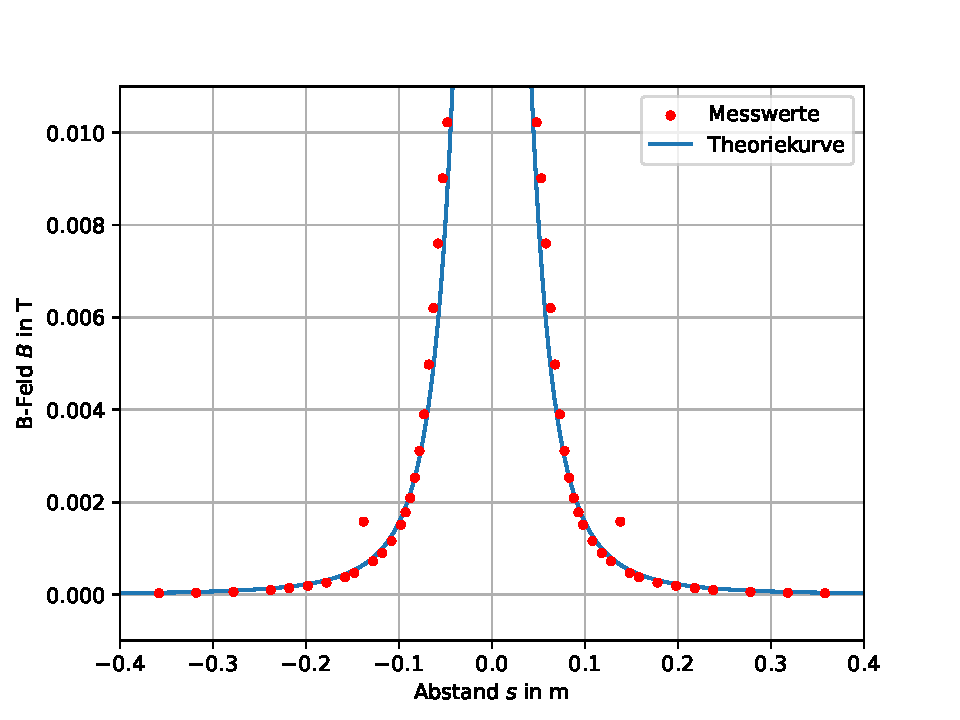
\includegraphics[width=0.8\textwidth]{mur.pdf}
        \caption{Fit der Permeabilitätsmessung}
        \label{fig:murfit}
    \end{figure}

    \subsection{transversale Konfiguration}
    Die gemessenen Daten der transversalen Konfiguration wurden im Graph \ref{fig:transmess} geplottet.
    Genauso wie bei der longitudinalen Konfiguration fällt das Magnetfeld mit größerem Abstand ab, beide fallen sogar ungefähr gleich schnell ab, nur ist erstaunlicherweise der Startwert der transversalen Messung mit $10 \si{\milli\tesla}$ direkt an der Seite der Spule größer als der Wert der longitudinalen Messung direkt in der Spule, der etwa $8 \si{\milli\tesla}$ beträgt.
    \begin{figure}[h]
        \centering
        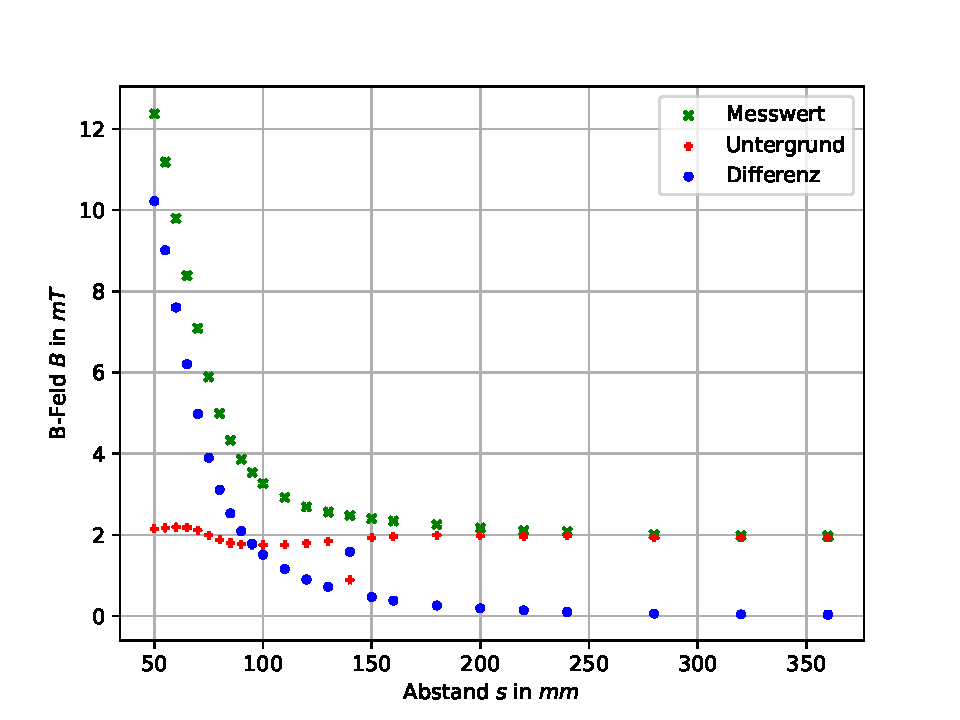
\includegraphics[width=0.8\textwidth]{raw2.pdf}
        \caption{Messwerte transversale Konfiguration}
        \label{fig:transmess}
    \end{figure}





    \section{Diskussion}

    \bibliographystyle{plain}
    \bibliography{literature}

\end{document}